\documentclass[a4paper, oneside, openany, dvipsnames, table]{article}
\usepackage[utf8]{inputenc}

\usepackage{lmodern}
\usepackage{breakurl}
\usepackage[T1]{fontenc}
\usepackage[italian]{babel}
\usepackage{stile}

\begin{document}
%Prima pagina
\copertina
%Indice
\tableofcontents
%Introduzione
\newpage
\section{Introduzione}
	Il progetto \emph{Pasticceria Padovana} vuole implementare un sito Internet che offra la possibilità di fornire informazioni riguardo il suo punto vendita.\\
Il sito Internet dovrà contenere informazioni riguardanti i prodotti disponibili, suddivisi in paste e torte, la storia della pasticceria, i contatti e l'ubicazione.\\
Il sito permette di inserire, modificare ed eliminare i prodotti: queste operazioni sono permesse solamente ad un utente privilegiato, mentre tutti gli altri utenti saranno visitatori 
normali a cui viene garantita la visualizzazione delle pagine del sito consentite.\\
Inoltre deve essere garantita l'accessibilità in modo che chiunque possa navigare nel sito serenamente.\\
Una volta garantita l'accessibilità, si vuole focalizzare l'attenzione sull'usabilità, rispettando gli standard W3C e la separazione tra struttura, presentazione e comportamento.\\
L'obiettivo del sito Internet è garantire una navigazione e ricerca fluida degli utenti all'interno del sito, in modo da evitare il disorientamento e, nel caso dovesse succedere, 
garantire supporto per tornare all'interno del sito.\\

%Analisi	
\newpage
\section{Analisi}
	\input{sezioni/Analisi.tex}
	\subsection{Studio dell'utenza finale}
		Il sito Internet si propone di fornire informazioni riguardanti la Pasticceria Padovana, ed è pensato per garantire una navigazione fluida con il minor numero di operazioni, per guardare e cercare i prodotti offerti dalla pasticceria.\\
Pertanto gli utilizzatori del sito appartengono ad una categoria di utenti omogenei: dai possibili clienti della pasticceria ai visitatori casuali del sito, fino ad arrivare ai dipendenti dell'attività.\\
Da evidenziare che questa categoria di utenti è esterna al sito è verrà denonimanata con la dicitura \emph{utente generico}.
L'unico utente che può attivare le funzionalità speciali del sito e che può essere considerato a tutti gli effetti un utente interno, viene chiamato \emph{amministratore} e lo diventa a tutti gli effetti dopo aver provveduto ad accedere alla zona riservata del sito tramite un form dedicato.\\
Quindi, l'utente finale è principalmente generico, e per questo è necessario utilizzare un linguaggioinformale, semplice e di facile intuizione, che possa essere compreso dalla maggior parte delle persone.\\ 
Lo stesso concetto vale per la struttura del sito e per il layout, che hanno l'obiettivo di fornire un modello mentale più familiare possibile all'utente, evitando di rompere le convenzioni esterne e, indipendentemente dalla strategia di browsing, rendendo veloce e intuitiva la navigazione all'interno del sito.\\
	\subsection{Casi d'uso}
		\input{sezioni/Analisi/casi_uso.tex}
		\subsubsection{Utente generico}
			L'utente viene definito \emph{generico} nel momento in cui può solo navigare nella pagina, senza alcun permesso di accedere all'area riservata.\\
L'utente generico dispone dei seguenti casi d'uso:
\begin{itemize}
	\item \hyperref[par:VisHome]{ Visualizzazione pagina "Home" (\ref{par:VisHome})};
	\item \hyperref[par:VisPaste]{ Visualizzazione pagina "Paste"(\ref{par:VisPaste})};
	\item \hyperref[par:CerPaste]{ Cerca prodotti in "Paste" (\ref{par:CerPaste})};
	\item \hyperref[par:VisTorte]{ Visualizzazione pagina "Torte" (\ref{par:VisTorte})};
	\item \hyperref[par:CerTorte]{ Cerca prodotti in "Torte" (\ref{par:CerTorte})};
	\item \hyperref[par:VisStoria]{ Visualizzazione pagina "Storia" (\ref{par:VisStoria})};
	\item \hyperref[par:VisContatti]{ Visualizzazione pagina "Contatti" (\ref{par:VisContatti})};
\end{itemize}

\paragraph{Visualizzazione pagina "Home"}\mbox{}\\
\label{par:VisHome}
L'utente generico può entrare nella pagina \emph{Home} in diversi modi:
\begin{itemize}
	\item se è appena entrato nel sito, è la prima pagina che viene visualizzata;
	\item se si trova in un'altra pagina, può raggiungere la homepage cliccando la sezione "Home" presente nel menu laterale;
	\item se si trova in un'altra pagina, può raggiungere la homepage cliccando sul logo presente nell'header;
\end{itemize}
All'interno di questa pagina l'utente può visualizzare una breve presentazione della pasticceria.\\

\paragraph{Visualizzazione pagina "Paste"}\mbox{}\\
\label{par:VisPaste}
L'utente generico può entrare nella pagina \emph{Paste} cliccando la sezione "Paste" presente nel menu laterale.
In questa pagina vengono visualizzate al massimo 10 paste alla volta. Ogni pasta conterrà un'immagine, il titolo e una descrizione.\\ 

\paragraph{Cerca prodotti in "Paste"}\mbox{}\\
\label{par:CerPaste}
Una volta entrato nella pagina \emph{Paste}, si potrà visualizzare una barra di ricerca posta all'inizio del content.\\
L'utente potrà cercare nella lista il prodotto desiderato inserendo il titolo, o una sottostringa del titolo, della pasta all'interno della barra di ricerca. Cliccando sul bottone \emph{cerca} visualizzerà instantaneamente le paste desiderate.

\paragraph{Visualizzazione pagina "Torte"}\mbox{}\\
\label{par:VisTorte}
L'utente generico può entrare nella pagina \emph{Torte} cliccando la sezione "Torte" presente nel menu laterale.
In questa pagina vengono visualizzate al massimo 10 torte alla volta. Ogni pasta conterrà un'immagine, il titolo e una descrizione.\\

\paragraph{Cerca prodotti in "Torte"}\mbox{}\\
\label{par:CerTorte}
Una volta entrato nella pagina \emph{Torte}, si potrà visualizzare una barra di ricerca posta all'inizio del content.\\
L'utente potrà cercare nella lista il prodotto desiderato inserendo il titolo, o una sottostringa del titolo, della torta all'interno della barra di ricerca. Cliccando sul bottone \emph{cerca} visualizzerà instantaneamente le torte desiderate.

\paragraph{Visualizzazione pagina "Storia"}\mbox{}\\
\label{par:VisStoria}
Attraverso questa pagina l'utente potrà visualizzare la storia della Pasticceria Padovana.\\
Vengono fornite informazioni riguardanti la nascita dell'azienda e l'evoluzione del laboratorio,
nonchè dei nostri pasticceri che da sempre deliziano il palato di moltissimi clienti.\\
Non mancano riferimenti ai prestigiosi premi vinti nel corso degli anni.

\paragraph{Visualizzazione pagina "Contatti"}\mbox{}\\
\label{par:VisContatti}
L'utente generico può entrare nella pagina \emph{Contatti} in diversi modi: se si trova in "Home","Paste","Torte","Storia"
\begin{itemize}
	\item cliccando la sezione "Contatti" presente nel menu laterale; 
	\item cliccando sul link \emph{Vieni a trovarci!} presente in un contenitore posto sotto il contenitore degli orari posto sotto il menu;
\end{itemize}
All'interno di questa pagina sono contenute le informazioni relative ai vari contatti aziendali (telefono e mail),
gli orari di apertura e l'ubicazione dell'attività su Google Maps.

		\subsubsection{Amministratore}
			L'utente \emph{amministratore} è l'unico utente addetto ad accedere all'area riservata: nessun altro può gestire il sito web, in quanto l'amministratore è l'unico utente ad avere le credenziali d'accesso.  Come richiesto dalle regole per la consegna del progetto, login e password sono uguali ad \textbf{admin}. Eredita tutti gli use case di \textit{utente generico}, e dispone di alcune funzionalità extra:
\begin{itemize}
	\item \hyperref[par:LoginAA]{ Login "Area Amministratore" (\ref{par:LoginAA})};
	\item \hyperref[par:AddP]{ Aggiungi prodotto in "Paste" (\ref{par:AddP})};
	\item \hyperref[par:ModP]{ Modifica prodotto in "Paste" (\ref{par:ModP})};
	\item \hyperref[par:DelP]{ Elimina prodotto in "Paste" (\ref{par:DelP})};
	\item \hyperref[par:AddT]{ Aggiungi prodotto in "Torte" (\ref{par:AddT})};
	\item \hyperref[par:ModT]{ Modifica prodotto in "Torte" (\ref{par:ModT})};
	\item \hyperref[par:DelT]{ Elimina prodotto in "Torte" (\ref{par:DelT})};
	\item \hyperref[par:ModN]{ Modifica la sezione "News" (\ref{par:ModN})};
	\item \hyperref[par:LogoutAA]{ Logout "Area Amministratore" (\ref{par:LogoutAA})};
\end{itemize}

\paragraph{Login "Area Amministratore"}\mbox{}\\
\label{par:LoginAA}
L'amministratore può accedere alla zona riservata \emph{Area Amministratore} inserendo le credenziali username e password e cliccando sul bottone \emph{Accedi} posto all'interno del form presente nel footer.\\ Nella versione mobile, il form si visualizzerà solo quando si cliccherà l'apposito bottone \emph{Accesso amministratore}: una volta cliccato, si aprirà il form con gli annessi bottoni \emph{Accedi} ed \emph{Esci} (per non visualizzare più il form).\\ Se le credenziali sono corrette, allora il login è andato a buon fine e si visualizzerà sul footer il form \emph{Benvenuto amministratore!} con il relativo bottone \emph{Esci}, altrimenti si visualizzerà una barra di colore rosso ad inizio finestra con un errore specifico:
\begin{itemize}
	\item se manca un campo da inserire od entrambi, il messaggio sarà \emph{Hai inserito simboli non consentiti};
	\item Se le credenziali inserite non sono corrette, il messaggio sarà \emph{Credenziali non corrette}.
\end{itemize}

\paragraph{Aggiungi prodotto in "Paste"}\mbox{}\\
\label{par:AddP}
L'amministratore può aggiungere una pasta alla volta, cliccando sul bottone apposito \emph{Aggiungi prodotto} nel content di "Paste".\\ Una volta cliccato, si ha accesso ad un form all'interno del content che conterrà i campi: \emph{Nome Prodotto}, \emph{Immagine prodotto} e \emph{Descrizione Prodotto}.\\ 
Una volta inseriti tutti i campi, allora si clicca sul bottone \emph{Modifica} e si viene reindirizzati alla pagina \emph{Paste} con il nuovo prodotto aggiunto all'elenco di paste in prima posizione.\\

\paragraph{Modifica prodotto in "Paste"}\mbox{}\\
\label{par:ModP}
L'amministratore può modificare una pasta alla volta cliccando sul bottone apposito \emph{Modifica prodotto}, che è associato ad ogni singola pasta.\\ 
Una volta cliccato il bottone, si ha accesso ad un form all'interno del content dove si potranno modificare i singoli campi della pasta in questione. Il testo è precompilato, ovvero che riprende tutto il contenuto della pasta.\\
Una volta cliccato il bottone \emph{Modifica}, allora si viene reindirizzati alla pagina "Paste" con l'elenco aggiornato.\\

\paragraph{Elimina prodotto in "Paste"}\mbox{}\\
\label{par:DelP}
L'amministratore può eliminare una pasta alla volta cliccando sul bottone apposito \emph{Elimina prodotto}, che è associato ad ogni singola pasta.\\ 
Una volta cliccato il bottone, la pasta viene eliminata una volta per tutte dalla pagina "Paste".\\

\paragraph{Aggiungi prodotto in "Torte"}\mbox{}\\
\label{par:AddT}
L'amministratore può aggiungere una torta alla volta, cliccando sul bottone apposito \emph{Aggiungi prodotto} nel content di "Torte".\\ Una volta cliccato, si ha accesso ad un form all'interno del content che conterrà i campi: \emph{Nome Prodotto}, \emph{Immagine prodotto} e \emph{Descrizione Prodotto}.\\ 
Una volta inseriti tutti i campi, allora si clicca sul bottone \emph{Modifica} e si viene reindirizzati alla pagina \emph{Torte} con il nuovo prodotto aggiunto all'elenco di torte in prima posizione.\\

\paragraph{Modifica prodotto in "Torte"}\mbox{}\\
\label{par:ModT}
L'amministratore può modificare una torta alla volta cliccando sul bottone apposito \emph{Modifica prodotto}, che è associato ad ogni singola torta.\\ 
Una volta cliccato il bottone, si ha accesso ad un form all'interno del content dove si potranno modificare i singoli campi della torta in questione. Il testo è precompilato, ovvero che riprende tutto il contenuto della torta.\\ 
Una volta cliccato il bottone \emph{Modifica}, allora si viene reindirizzati alla pagina "Torte" con l'elenco aggiornato.\\

\paragraph{Elimina prodotto in "Torte"}\mbox{}\\
\label{par:DelT}
L'amministratore può eliminare una torta alla volta cliccando sul bottone apposito \emph{Elimina prodotto}, che è associato ad ogni singola torta.\\ 
Una volta cliccato il bottone, la torta viene eliminata una volta per tutte dalla pagina "Torte".\\

\paragraph{Modifica la sezione "News"}\mbox{}\\
\label{par:ModN}
L'amministratore può modificare la sezione \emph{News}, posta sotto il menu laterale, cliccando il bottone \emph{Modifica news}.\\ 
Una volta cliccato, si ha accesso ad un form all'interno del content dove si potranno modificare i campi \emph{Titolo News} e \emph{Descrizione News}.\\
Concluse le modifiche, si clicca il bottone "Modifica" e si verrà reindirizzati alla pagina precedente, con la sezione "News" aggiornata.\\

\paragraph{Logout "Area Amministratore"}\mbox{}\\
\label{par:LogoutAA}
L'amministratore può fare logout dalla zona riservata cliccando sul bottone \emph{Esci} posizionato nel footer.\\ Una volta cliccato, ricomparirà il form per l'accesso all'area amministratore e si ritorna in modalità \emph{utente generico}.\\
%Progettazione
\newpage
\section{Progettazione}
	\input{sezioni/Progettazione.tex}
	\subsection{Obiettivi}
		Il progetto \emph{Pasticceria Padovana} si prefigge di rispettare le specifiche tecniche richieste, in particolare:
\begin{itemize}
	\item \textbf{Separazione tra contenuto, presentazione e comportamento:} primo requisito fondamentale. 
	Il contenuto è stato progettato in modo statico in XHTML 1.0, la presentazione in CSS3 e il comportamento è gestito in modo dinamico con PHP7 e JavaScript.\\
	E' stato scelto di non progettare il contenuto in HTML5 per il fatto che HTML5 non ha raggiunto la piena compatibilità con i browser attualmente in circolazione.\\
	\item \textbf{Accessibilità:} tutte le categorie di utenti devono poter utilizzare il sito senza particolari ostacoli.\\ 
	Il sito è stato costruito per organizzare i propri contenuti in modo da poter essere facilmente reperiti da qualsiasi utente, 
	in modo da non generare disorientamento e sovraccarico cognitivo.\\ 
	Le implementazioni più importanti sono:
	\begin{itemize}
		\item attributo \emph{alt} nelle immagini, che rende disponibile un testo alternativo in caso in cui l'immagine non venga caricata.\\ 
		Il testo alternativo deve essere coerente con l'immagine visualizzata: se è un'immagine decorativa e priva di significato si inserisce un testo vuoto, 
		altrimenti si scrive una breve descrizione.
		\item link \emph{Salta il contenuto}, nascosto di default ma visibile agli screen reader. E' la prima voce del menu, viene utilizzata nel caso in cui l'utente che
		utilizza lo screen reader voglia saltare direttamente al contenuto della pagina, velocizzando la navigazione.\\
		\item link {torna su}, sotto forma di bottone circolare sempre visibile, che si trova a lato del content: se invocato, ti porta all'inizio del content. 
		Utile per evitare lo scroll e velocizzare la navigazione.
		\item utilizzo della tecnologia \emph{WAI-ARIA}: abbinata ad XHTML nel doctype, è stata implementata per migliorare la lettura degli screen reader.\\
		I comandi più utilizzati sono: \emph{aria-hidden="true"}, che impedisce che un elemento venga letto dal lettore di schermo, e \emph{aria-label="..."}, 
		che legge il testo presente in aria-label quando il campo riceve il focus. 
		\item buon contrasto dei colori, verificato per sopperire ai noti problemi dell'ipovedenza.\\
		\item le parti più rilevanti del sito sono inserite nella comfort zone: per esempio, il menu ad hamburger presente nella versione mobile si posiziona in una zona 
		facilmente raggiungibile dal pollice della mano destra, al pari del contenuto della pagina.\\
	\end{itemize}
	\item \textbf{Usabilità:} tutti gli utenti possono ottenere quello che vogliono dal sito in un tempo ragionevole e in modo piacevole. E' la conseguenza dell'accessibilità: 
	non ci può essere usabilità senza accessibilità.\\ 
	\item \textbf{Punti di rottura del layout:} applicati per rendere flessibile il sito ai cambiamenti della risoluzione dello schermo, da quelli desktop a quelli mobile.\\
	I punti di rottura sono definiti in css come: \emph{@media only screen and (min-width: ...px) }.
	\item \textbf{Comprensibilità delle informazioni:} le informazioni presentate nel sito sono di semplice comprensione e mirate ad essere esaustive.\\
\end{itemize}
	\subsection{Design del sito}
		La strategia di progettazione del design che è stata implementata è \emph{Responsive Web Design}.\\
Questa tecnica è incentrata sull'accessibilità e permette la realizzazione del sito in modo che si possa adattare graficamente in modo automatico al tipo di device che si sta utilizzando.\\ 
Il layout che è stato scelto è un \emph{layout a cinque pannelli}, che si adatta facilmente al concetto di \emph{Responsive Web Design}.\\
I pannelli presenti nel layout sono, in ordine di presentazione:
\begin{enumerate}
	\item \textbf{header:} contiene il logo della pasticceria e un titolo che descrive la pagina corrente;
	\item \textbf{breadcrumb:} contiene il percorso della pagina corrente, serve ad orientare l'utente all'interno del sito;
	\item \textbf{menu:} contiene le varie sezioni del sito: quella corrente appare in grassetto, mentre le sezioni già visitate sono contrassegnate in viola. Inoltre, sotto le voci del menu corrispondenti alle sezioni, 
	appaiono due box con informazioni relative alle news e agli orari della pasticceria;
	\item \textbf{content:} contiene il contenuto della pagina corrente;
	\item \textbf{footer:} contiene le informazioni riguardo i contatti, gli orari della pasticceria, il form per accedere all'\emph{Area Amministratore}, i progettisti del sito, il copyright e gli standard rispettati.
\end{enumerate}

\newpage
Il layout si presenta in modi diversi, in base alle dimensioni dello schermo sulla quale l'utente sta navigando:\\
\begin{itemize}
	\item
	\textbf{Versione desktop}\\ 
	\begin{figure}[!h]
		\centering
		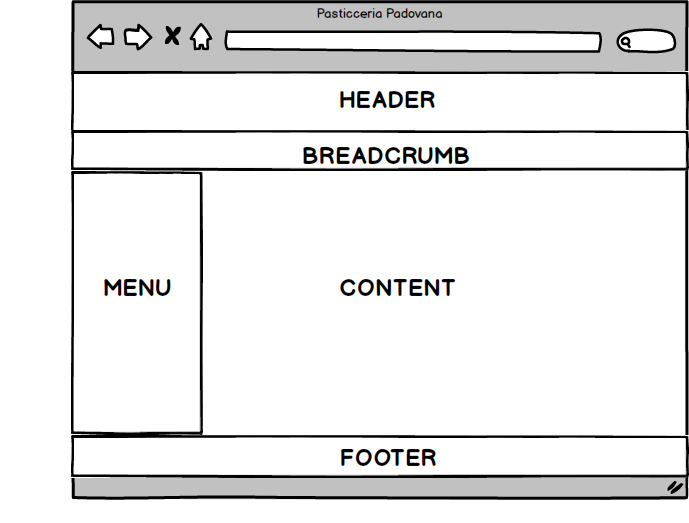
\includegraphics[width=0.7\linewidth]{sezioni/Progettazione/Immagini/desktop_layout.png}
	    \caption{Layout di una pagina in versione desktop}
		\label{Fig:verDesktop}
	\end{figure}
	\item	  
	\textbf{Versione mobile}	
	\begin{figure}[!h]				  
		\centering
		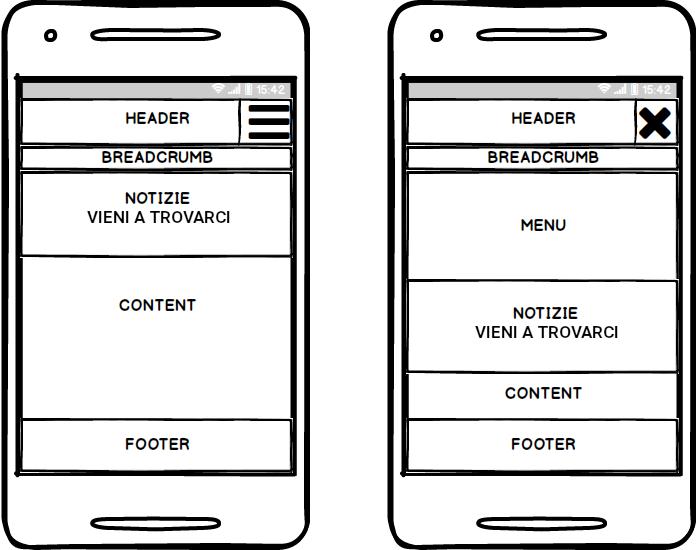
\includegraphics[width=0.7\linewidth]{sezioni/Progettazione/Immagini/mobile_layout.png}
	    \caption{Layout di una pagina in versione mobile: menu chiuso(sinistra) e menu aperto(destra)}
	    \label{Fig:verMobile}
	\end{figure}	  
\end{itemize}
\newpage	

	\subsection{Database}
		Un'altra parte fondamentale del progetto è il database, in quanto il sito si appoggia su di esso per richiedere parti del contenuto informativo.\\ 
In fase di progettazione, è stato pensato di creare un database con la funzione di contenere tutti i dati relativi ai prodotti in vendita, ovvero \emph{paste} e \emph{torte}, 
e al contenuto del contenitore \emph{news}.\\
Come si può vedere dalla \emph{Figura \ref{Fig:schemadb}}, le tabelle (che rappresentano sià entità che associazioni e i loro relativi attributi chiave/non chiave) sono quattro:
\begin{itemize}
		\item \textbf{Prodotto:} contiene tutti i dati relativi ai prodotti che verranno visualizzati nelle pagine \emph{Paste} e \emph{Torte}
		\item \textbf{Recensione:} contiene tutti i dati riguardo al feedback rilasciato da un utente per un prodotto specifico
		\item \textbf{Utente:} contiene i dati di tutti gli utenti che sono registrati al sito della pasticceria
		\item \textbf{News:} contiene tutti i dati addetti a riempire la sezione \emph{News} sotto il menu 
\end{itemize}
\begin{figure}[!h]
	\centering
	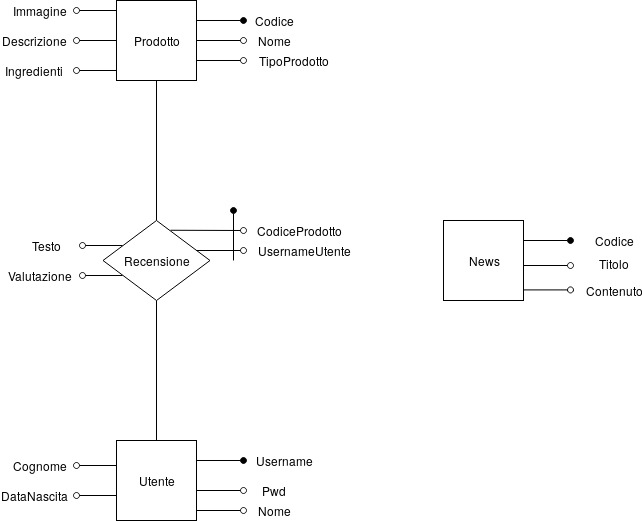
\includegraphics[width=0.7\linewidth]{sezioni/Progettazione/Immagini/schema_concettuale.jpg}\\
    \caption{Schema concettuale database}
	\label{Fig:schemadb}
\end{figure}
Ai fini di questo progetto, per vari motivi che sono stati discussi all'interno del gruppo, tre delle quattro tabelle elencate sono utilizzate nel momento in cui PHP interviene per 
prelevare i dati di interesse dal database.\\
Come spiegato nella sezione \emph{Analisi}, esistono due tipi di utenti in questo progetto: \emph{utente generico} e \emph{amministratore}.\\ L'utente generico non viene salvato nella 
tabella \emph{Utente}, in quanto non ha bisogno di registrarsi al sito per la semplice navigazione, mentre l'amministratore deve avere le credenziali appposite per entrare 
nell'\emph{Area amministratore}.\\
Inoltre, è obbligatorio l'utilizzo della tabella \emph{News} per visualizzare le novità della pasticceria, e della tabella \emph{Prodotto} per poter visualizzare paste e torte, in quanto 
i dati sono richiesti dinamicamente (altrimenti le pagine sarebbero vuote).\\
Ergo, la tabella \emph{Recensione} può servire solo nel caso in cui si vuole aggiungere un servizio interno al sito che prevede la registrazione di utenti che possono scrivere recensioni 
per i prodotti della pasticceria. Quindi, ai fini degli obiettivi del nostro progetto, la tabella è stata creata con l'intento di averla pronta per implementazioni future.\\
Stesso discorso si applica alla tabella \emph{Utente}: in questo progetto, questa tabella sarà riempita solamente con i dati dell'amministratore, in quanto unico utente ad aver accesso 
all'\emph{Area amministratore} implementata nel sito.\\
Nel momento in cui si vorrà implementare il servizio di recensioni utente, allora la tabella sarà composta anche dai parametri degli utenti che si registrano al servizio mediante pagina 
di registrazione (non prevista in questo progetto).


%Presentazione
\newpage
\section{Presentazione}
	Il foglio di stile implementato garantisce un design fluido e scalabile, grazie all'utilizzo di unità di misura
sempre relative o in percentuale. \\Questo migliora l'accessibilità e garantisce una corretta visualizzazione delle pagine
su tutti i formati di schermi. \\Il sito dispone di 4 modalità di visualizzazione differente: desktop, tablet, mobile e di stampa.

\subsection{Desktop}
La versione desktop è stata pensata in modo da avere una navigazione estremamente semplice.\\ 
Nella colonna di sinistra sono presenti anche le \emph{news}, ed una sezione \emph{vieni a trovarci} con gli orari di apertura della pasticceria.\\ 
Da notare la larghezza massima impostata a 1200px, che permette agli utenti di utilizzare il sito con una finestra ridotta su schermi di certe dimensioni.

\begin{figure}[!h]
	\centering
	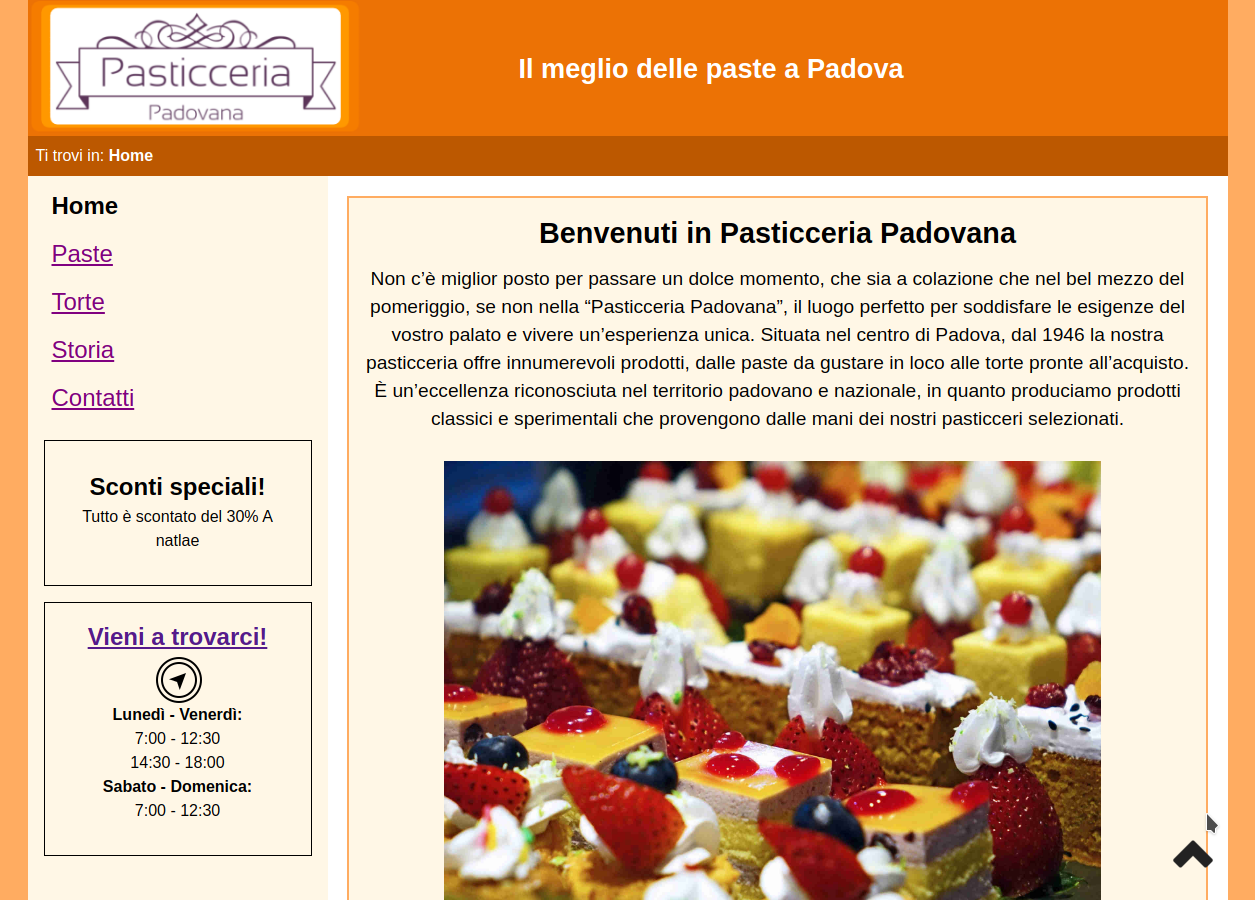
\includegraphics[width=1\linewidth]{sezioni/Progettazione/Immagini/desktop_example.png}
	\caption{Esempio di una pagina in versione desktop}
	\label{Fig:verDesktop}
\end{figure}
\newpage
\subsection{Tablet}
La versione tablet implementa l'interfaccia in modo diverso. Dato lo spazio limitato dello schermo, il gruppo ha deciso di implementare
un menù ad hamburger. Anche le \emph{news} non sono più laterali, ma si trovano in cima al contenuto della pagina. In questo modo viene data
maggiore importanza alle \emph{news} e agli orari della pasticceria, cosa necessaria nei dispositivi portatili.\\
Anche il form di login da parte dell'amministratore nelle versioni mobili è stato nascosto e reso disponibile tramite un bottone.
\begin{figure}[!h]		
    \centering		  
	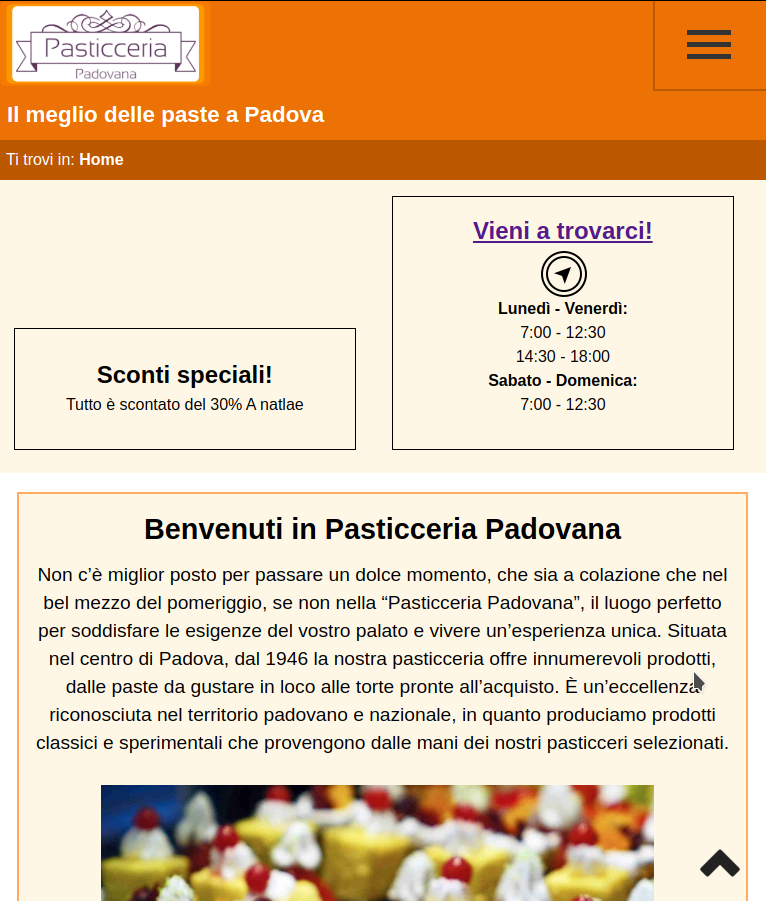
\includegraphics[width=0.8\linewidth]{sezioni/Progettazione/Immagini/tablet_example.png}
	\caption{Esempio di una pagina in versione tablet}
	\label{Fig:verTablet}
\end{figure}	    
\newpage

\subsection{Mobile}
La versione mobile differisce di molto poco rispetto alla versione tablet. Solo \emph{news} e sezione \emph{vieni a trovarci} con orari sono state poste incolonnate invece che affiancate.
\begin{figure}[!h]
    \centering		  
	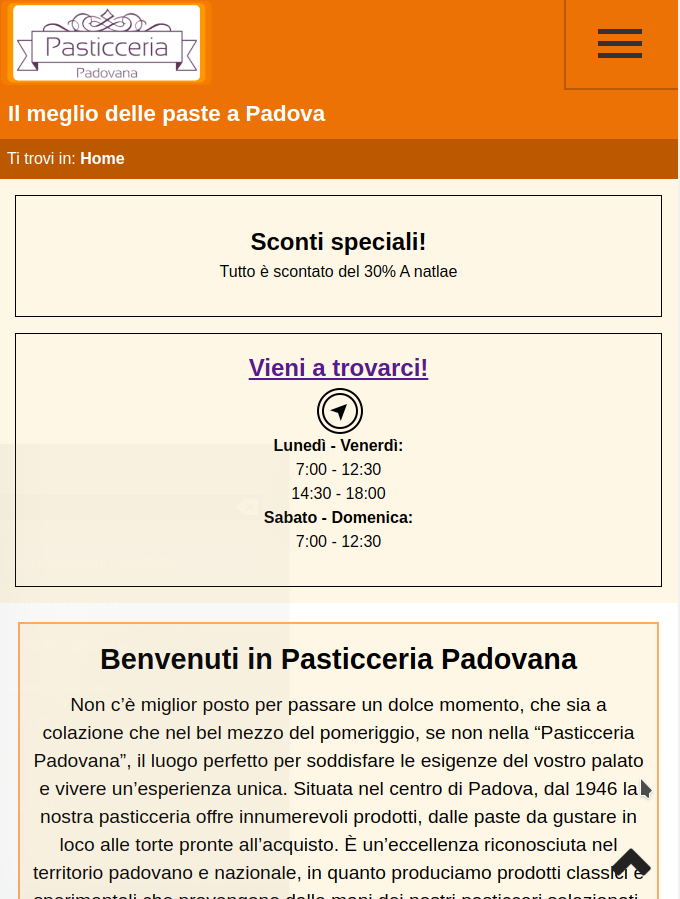
\includegraphics[width=0.8\linewidth]{sezioni/Progettazione/Immagini/mobile_example.png}
	\caption{Esempio di una pagina in versione mobile}
	\label{Fig:verMobile}
\end{figure}
\newpage

\subsection{Print}
La stampa elimina tutte le funzionalità interattive. In questo modo una pagina stampata conterrà solamente il contenuto interessato.\\
Vengono quindi eliminati la maggior parte degli stili, dei colori e delle immagini in quanto l'obbiettivo di una stampa è ottenere un foglio 
contenente solo informazioni realmente utili.\\
La scelta è stata quella di mantenere le foto ai prodotti nella stampa. Questo poichè la presentazione dei prodotti di una pasticceria è di rilevante importanza.\\
\begin{figure}[!h]
    \centering		  
	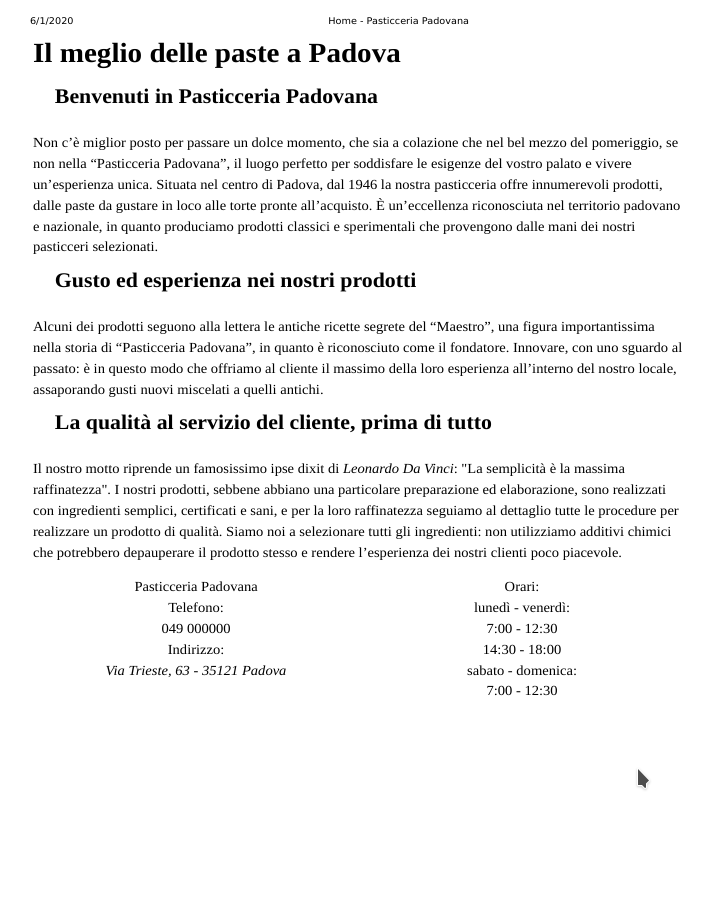
\includegraphics[width=0.8\linewidth]{sezioni/Progettazione/Immagini/print_example.png}
	\caption{Esempio di una stampa}
	\label{Fig:verPrint}
\end{figure}


\newpage
%Implementazione
\newpage
\section{Implementazione}
	\input{sezioni/Implementazione.tex}
	\subsection{Linguaggi}
		\input{sezioni/Implementazione/linguaggi.tex}
		\subsubsection{XHTML e CSS3}
			Il sito da noi realizzato è stato pensato per un'utenza assolutamente non all'avanguardia per quanto riguarda la tecnologia.\\
Proprio per questo è stato scelto di utilizzare \emph{XHTML}, in modo da garantire il funzionamento totale del sito in ogni ambiente, ma anche in modo da
avere una sintassi più rigida in fase di implementazione.\\ Inoltre, per la realizzazione non è stato necessario utilizzare funzionalità aggiuntive
di \emph{HTML5}, quindi il passaggio ad HTML5 mantenendo la sintassi \emph{XHTML} non è stato necessario.\\
Sono state seguite le linee guida del \emph{W3C}, oltre che le spiegazioni in aula.\\
Il linguaggio di stile utilizzato è il \emph{CSS3}. Molto importante da sottolineare è il mantenimento di una separazione tra struttura e presentazione, che 
si manifesta: 
\begin{itemize}
    \item mantenendo i compiti dei due linguaggi separati, ovvero non utilizzando tag di stile in XHTML;
    \item separando il più possibile XHTML e CSS3, quindi senza implementare il codice a cascata inline o embedded ad XHTML, ma solo su file esterni.
\end{itemize}
Ogni singola regola CSS2 o CSS3 è stata valutata prima di utilizzarla, in base alla compatibilità dei browser.
Qualche regola CSS3 non è compatibile con IE8 causando una trasfomazione elegante.



		\subsubsection{PHP}
			Il gruppo ha deciso di elaborare le pagine server-side tramite il linguaggio \emph{PHP}. Questa operazione è necessaria, in quanto ogni pagina deve specializzarsi in base 
al tipo di utenza.\\
Il linguaggio \emph{PHP} consente di leggere e scrivere nel database, oltre che eseguire operazioni sul filesystem quali inserimento e cancellazione delle foto dei prodotti.\\
Importante è sottolineare la separazione tra struttura e comportamento, il cui significato e dimostrazione sarà nelle prossime righe.\\
Il sito internet è principalmente strutturato in questo modo: 
\begin{itemize}
    \item un file \emph{template.html} contenente tutte le parti statiche condivise da tutte le pagine;
    \item dei file \emph{'pagina'.php} le quali elaborano il contenuto del template in infine ritornano la pagina modificata;
    \item dei file \emph{storia.html, home.html} e \emph{contatti.html} usati dalle corrispondenti pagine php per recuperare le parti statiche;
    \item classi php per l'elaborazione e stampa delle parti più dinamiche, come il menù o la pagina dei prodotti;
    \item classi php per l'elaborazione di dati per il database o il salvataggio (o eliminazione) delle immagini;
\end{itemize}
Così facendo il ruolo del \emph{PHP} non sarà quello di andare a modificare la struttura della pagina, ma quel compito verrà lasciato ad \emph{XHTML}.\\
Il \emph{PHP} si occupa di elaborare informazioni e modificare quello che è il contenuto della pagina, ma non la sua struttura.\\


Viene lasciato al lato server un ulteriore controllo di sicurezza sugli input dell'utente. Banalmente, un utente avanzato potrebbe alterare il comportamento
del \emph{JavaScript} per oltrepassare i controlli, ma non potrà mai modificare il comportamento \emph{PHP} poichè è codice server-side.\\
Per questo è fornita una classe \emph{Input\_security\_check} contenente tutti i metodi necessari ai vari controlli, che operano controllando i singoli caratteri in input.
\begin{itemize}
    \item Il metodo \emph{general\_controls(input)} esegue operazioni fondamentali per quanto riguarda la sicurezza. Dato un input il metodo si occupa di passarlo tramite una serie di tre funzioni: 
    \begin{itemize}
        \item \emph{trim()}: elimina gli spazi prima e dopo la stringa in input;
        \item \emph{htmlentities()}: converte tutti i possibili caratteri in entità \emph{HTML};
        \item \emph{strip\_tags()}: elimina tutti i possibili tag \emph{HTML} all'interno;
    \end{itemize}
    \item I metodi \emph{username\_check()} e \emph{password\_check}, dopo aver richiamato il metodo di controllo generale si occupano di verificare se i possibili caratteri in input sono stati rispettati;
    \item Il metodo \emph{general\_input\_check()} dopo aver richiamato il metodo di controllo generale si occupa di aggiungere uno slash a tutti i caratteri che potrebbero influire all'esecuzione di una query tramite la funzione \emph{addslashes()};
\end{itemize}

Test di query injection saranno descritti nella sezione test.AA
		\subsubsection{SQL}
			Per il salvataggio dei dati il gruppo, ha deciso di utilizzare SQL tramite \emph{MariaDB}.\\
Per eseguire le interrogazioni o aggiornare il database, è stata usata la libreria \emph{mysqli} di \emph{PHP}.\\
Il database collegato al sito è molto semplice, ed è descritto nel capitolo 3: \emph{Progettazione -> Database}.

		\subsubsection{JavaScript e AJAX}
			\emph{JavaScript} è un linguaggio che si occupa del comportamento del sito. Nel nostro caso specifico, il suo principale uso è rivolto dai controlli 
input lato client, dove ognuno di essi viene controllato prima di essere spedito, in modo da evitare elaborazioni inutili da parte del server.\\
Va evidenziato che i controlli client-side sono speculari ai controlli server-side, a parte qualche controllo aggiuntivo \emph{database-safe}.\\
L'utilizzo di JavaScript è importante anche per le animazioni del sito. Nel nostro progetto, le uniche animazioni da gestire sono implementate 
lato mobile, in quanto sono presenti alcuni elementi a comparsa.\\
La motivazione di questa scelta è molto semplice ed è giustificata dalla dimensione dello schermo, dove uno schermo mobile è più piccolo di uno schermo
in modalità desktop, quindi gli elementi da considerare devono occupare poco spazio, non essere invasivi ed essere essenziali ai fini dell'utente. \\
Quindi, è stato scelto di implementare:
\begin{itemize}
    \item un menù ad hamburger che mostra/nasconde le singole voci, rimpiazzando così il menu laterale lato desktop;
    \item un bottone \emph{Accesso amministratore} nel footer che, una volta premuto, fa comparire il form di login per l'amministratore, e per farlo
    scomparire può premere sul bottone \emph{Esci.} 
\end{itemize}    

La validazione dell'utente nel form di login avviene attraverso \emph{AJAX}, acronimo di \emph{Asynchronous JavaScript and XML}.\\ 
La motivazione di tale scelta è per il messaggio d'errore in caso di input scorretto: il form di login si trova nel footer, e nel caso di errore 
verrebbe inserito un messaggio d'errore dopo il ricaricamento della pagina, il che è scomodo perchè non si avrebbe accesso diretto ai campi del form
se non scrollando la pagina.\\
Grazie ad AJAX, l'errore viene visualizzato all'interno del form e la pagina non viene ricaricata.\\
Nel caso i vecchi browser non riescano a supportare questa funzionalità, visualizzeranno comunque lo stesso messaggio di errore, ma si dovrà scrollare la pagina.\\
AJAX entra in funzione nel momento in cui avviene un click nel submit. L'evento, reso asincrono, si occuperà in primo luogo di controllare 
se le credenziali sono corrette: se non lo sono, viene disabilitato il comportamento standard del submit, per visualizzare 
un messaggio d'errore.\\
%Validazione
\newpage
\section{Validazione}
	Questa sezione ha l'obiettivo di elencare e descrivere l'utilizzo degli strumenti utilizzati nell'ambito della validazione delle pagine.\\ 
La validazione è uno dei requisiti più sottovalutati, ma in realtà è uno dei più importanti, in quanto garantisce che il codice scritto sia corretto e di qualità, perchè conforme agli standard W3C.\\
I vantaggi della validazione di un sito web sono molteplici:
\begin{itemize}
	\item un sito è più accessibile se viene validato;
	\item se il codice è allineato con lo standard, permette di limitare le differenze di visualizzazione del sito da un browser all'altro e garantirne la compatibilità;
	\item la presenza di errori nella pagina rallenta la lettura da parte dei browser, pena un peggioramento della navigazione e dell'esperienza utente;
	\item la validazione di un sito influenza la sua indicizzazione ed il suo posizionamento sui vari motori di ricerca, pena meno traffico nel proprio sito web.  
\end{itemize}
Gli strumenti di validazione utilizzati nel corso del progetto sono i seguenti:
\begin{itemize}
	\item \textbf{W3C HTML Validator}\\
	Indirizzo sito web: \emph{https://validator.w3.org/}\\
	Servizio di validazione gratuito di W3C che consente di validare il codice (X)HTML.\\ 
	Inizialmente, la validazione era più instantanea in quanto era presente solo codice che generava pagine statiche ((X)HTML).\\Dal momento in cui è stato scritto codice che genera pagine dinamiche (PHP), allora si è provveduto a incollare l'intero codice sorgente in una sezione dedicata nel sito.\\
	Se il codice non è valido, segnala il numero di errori, il tipo di errori e a quale riga e colonna della pagina sono stati trovati.
	\item \textbf{W3C CSS Validator}\\
	Indirizzo sito web: \emph{https://jigsaw.w3.org/css-validator/}\\
	Servizio di valutazione gratuito di W3C che consente di validare il codice CSS.\\
	In questo caso basta scegliere il file CSS dalla directory e validarlo nell'apposita sezione.\\
	Con questo servizio è possibile validare il file (X)HTML con CSS integrato, ma non è il nostro caso in quanto, come richiesto dalle regole di progetto, \emph{il sito web deve rispettare la completa separazione tra contenuto, presentazione e comportamento}. 
\end{itemize}

 
%Fase di test
\newpage
\section{Fase di Test}
	La fase di test è l'attività di verifica del sito in tutti i suoi dettagli implementativi.\\ 
Sebbene questa attività venga fatta dopo la validazione (che deve essere corretta), la fase di test non è ultima per importanza, in quanto
senza essa non verrebbe assicurata l'accessibilità e l'usabilità del sito.\\
Ergo, la fase di test assume un importanza tale da non poter essere ignorata.\\
Di seguito verranno elencati gli strumenti di testing utilizzati per questa importante attività.

	\subsection{Audits}
		Sezione di \emph{Strumenti per sviluppatori} del browser Google Chrome.\\
Permette di identificare e risolvere i problemi inerenti alle performance del sito, all'accessibilità, all'esperienza utente e la SEO (Search Engine Optimization).\\
E' possibile verificare il sito da dispositivo mobile o desktop, e selezionare le varie verifiche. Nel nostro caso, la verifica \emph{Progressive Web App} non ci interessa in quanto il nostro progetto non è un applicazione Web che si carica come una normale pagina Web, ma un semplice sito Web.\\
Cliccando \emph{Run audits}, si accede al pannello dove vengono visualizzati i risultati in percentuale e le possibili correzioni da attuare.
\begin{figure}[!h]
	\centering
	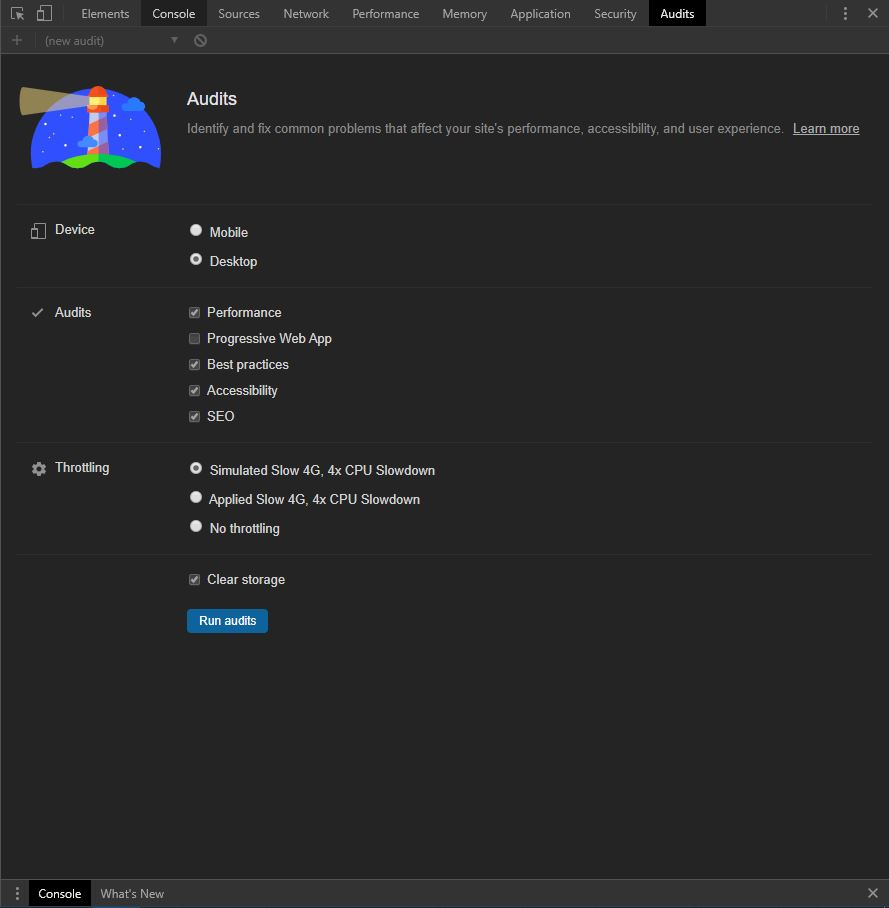
\includegraphics[width=0.7\linewidth]{sezioni/FaseTest/Immagini/audits.JPG}\\
	\caption{Strumenti per sviluppatori Google Chrome: Audits}
	\label{Fig:audits}
\end{figure}

\newpage
	\subsection{Silktide – disability simulator}
		Plugin del browser Google Chrome, che permette di navigare il sito dal punto di vista di una persona affetta da una particolare disabilità.\\
\begin{itemize}
	\item Può simulare uno screen reader, in modo da poter capire se il sito è accessibile o meno.
	\item Può simulare la visualizzazione del sito da parte di una persona miope, con parziale cecità oppure dislessia.
	\item Può simulare la visualizzazione del sito da parte di una persona che soffre di daltonismo, ovvero che ha un'alterata percezione dei colori.
\end{itemize}
L'obiettivo è rendere accessibile il sito a più categorie di utenti possibili. Ogni tipo di disabilità ha le sue sfacettature, e per questo motivo 
raggiungere tutti gli utenti può sembrare arduo se non impossibile, ma grazie a questi strumenti gli sviluppatori possono perfezionare i dettagli
implementativi del codice.
\begin{figure}[!h]
	\centering
	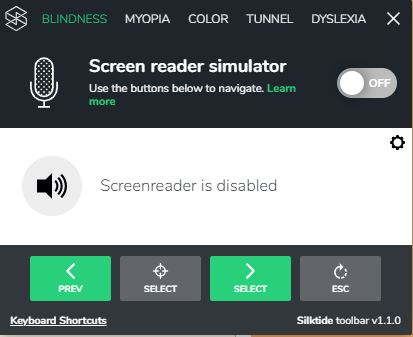
\includegraphics[width=0.7\linewidth]{sezioni/FaseTest/Immagini/screen_reader_simulator.JPG}\\
	\caption{Silktide – disability simulator : screen reader simulator}
	\label{Fig:silktide}
\end{figure} 
	\subsection{NVDA}
		Acronimo di \emph{Non Visual Desktop Access}, è un software gratuito ed opensource che consente alle persone con disabilità alla vista di utilizzare un computer autonomamente.\\ 
Installato su un sistema operativo Windows 10, NVDA legge qualsiasi contenuto del sistema operativo, non solo un generico browser.\\ 
Si utilizza tramite tastiera ed è molto veritiero, in quanto è uno strumento progettato per queste particolari evenienze.\\
Riferimento al sito: https://www.nvda.it/

\newpage
	\subsection{Web Developer}
		Plugin del browser Mozilla Firefox, permette di attuare modifiche instantanee sugli stili, le immagini, i form eccetera.\\
Strumento molto utile per capire come viene visualizzata una pagina in caso in cui alcuni elementi non vengano caricati (p.e. come si visualizza l'alt di un'immagine se questa non viene caricata). 
\begin{figure}[!h]
	\centering
	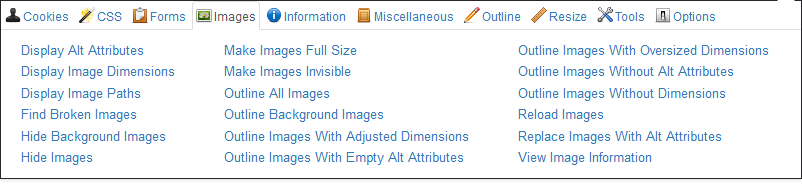
\includegraphics[width=0.7\linewidth]{sezioni/FaseTest/Immagini/web_developer.png}\\
	\caption{Web Developer - Images}
	\label{Fig:webDev}
\end{figure} 
	\subsection{Links2}
		\emph{Links2} è un browser testuale da terminale. Permette di visualizzare il sito solo con una struttura molto minimale. \\
Per garantire una buona navigazione generale, da parte di tutti, deve essere possibile utilizzare il sito anche tramite un browser testuale.\\
Quindi, se è possibile navigare facilmente con links2 allora la probabilità che una persona con disabilità visive abbia difficoltà a navigare
all'interno del sito scende di molto. Infatti tramite links2 sappiamo determinare anche il comportamento di uno screen reader.\\
Questo tool inoltre ci ha permesso di capire il comportamento del sito in mancanza di immagini.\\

\begin{figure}[!h]
	\centering
	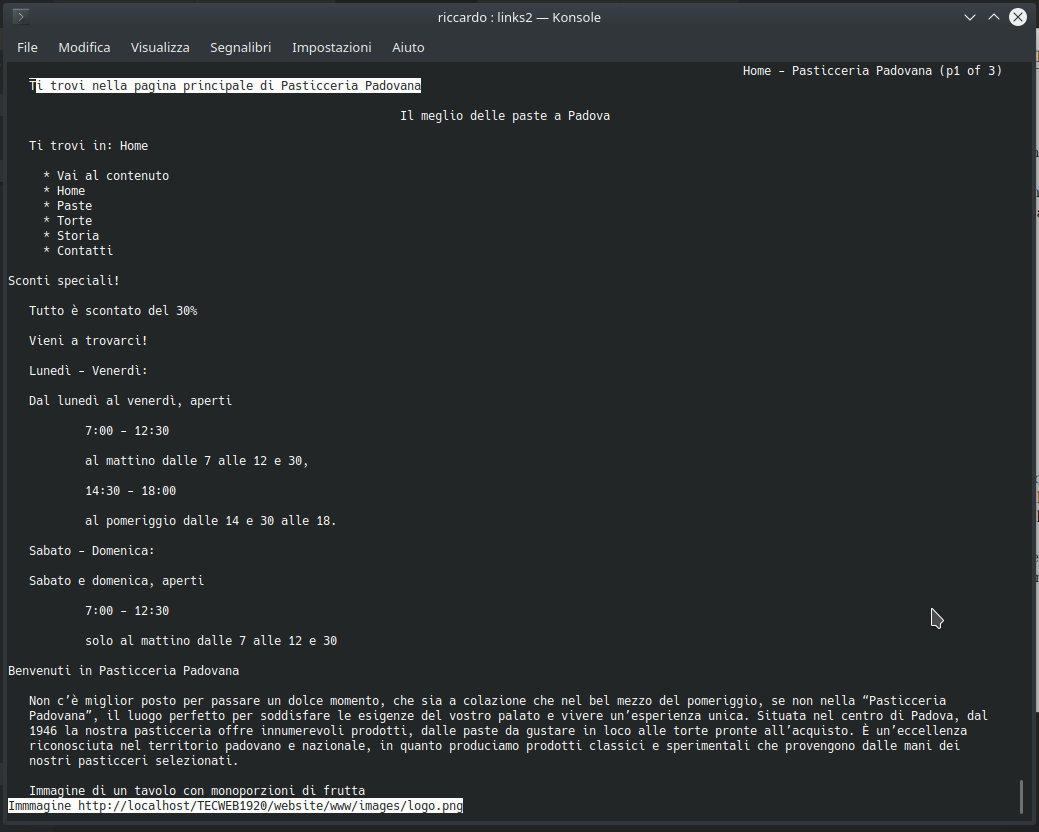
\includegraphics[width=0.7\linewidth]{sezioni/FaseTest/Immagini/links2.png}\\
	\caption{links2 – terminal browser}
	\label{Fig:links2}
\end{figure} 
\newpage
	\subsection{XAMPP}
		\emph{XAMPP} è una distribuzione di Apache contenente MySQL, PHP e Perl, ed è un pacchetto open source che, ai fini del progetto, ha permesso
al team di sviluppo di testare in locale la parte dinamica del sito, in modo da simulare l'elaborazione delle richieste PHP e delle 
interrogazioni SQL come se il nostro sito funzionasse all'interno di un server remoto.\\
\begin{figure}[!h]
	\centering
	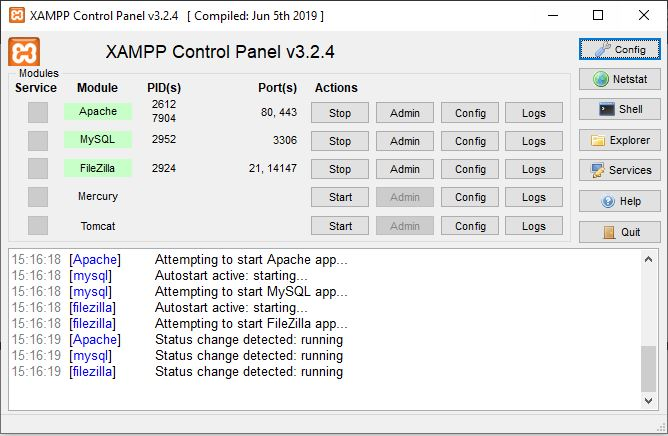
\includegraphics[width=0.7\linewidth]{sezioni/FaseTest/Immagini/xampp.JPG}\\
	\caption{XAMPP Control Panel}
	\label{Fig:xampp}
\end{figure} 
%Suddivisione del lavoro
\newpage
\section{Suddivisione del lavoro}
	In questa sezione viene specificato il lavoro effettuato dai vari membri del gruppo:
\begin{itemize}
	\item \textbf{Alberto Gobbo}
	\begin{itemize}
		\item Struttura iniziale e sviluppo del codice HTML
		\item Struttura iniziale e qualche parte di CSS, parte desktop 
		\item Stesura della relazione, eccetto parte \emph{Implementazione})
		\item Validazione delle pagine
	\end{itemize}	
	\item \textbf{Marco Dalla Libera}
	\begin{itemize}
		\item Struttura iniziale e sviluppo del codice HTML
		\item Struttura iniziale e sviluppo del codice CSS, parte mobile
		\item Sviluppo del codice JavaScript
	\end{itemize}	
	\item \textbf{Riccardo Cestaro}
	\begin{itemize}
		\item Struttura iniziale e sviluppo del codice HTML
		\item Struttura iniziale e sviluppo del codice CSS, parte desktop
		\item Sviluppo del codice PHP e implementazione AJAX
		\item Stesura sezione \emph{Implementazione} della relazione
	\end{itemize}	
	\item \textbf{Stefano Lazzaroni}
	\begin{itemize}
		\item Sviluppo del codice PHP
		\item Fase di verifica sui file CSS, sia screen che print
		\item Fase di test 
	\end{itemize}	
\end{itemize}

A parte qualche omissione, causa brevi modifiche del codice, ogni membro del gruppo è stato presente su ogni parte del codice.\\
Il lavoro da fare è stato suddiviso nella repository di GitHub, dove venivano create \emph{issue} ad ogni attività da svolgere e ad ogni nuova problematica.\\
Le issue venivano assegnate, auto-assegnate oppure lasciate senza un assegnatario in modo che chiunque potesse prendersi il carico della attività specifica da svolgere.\\
Le comunicazioni interne sono avvenute tramite gruppo di Whatsapp, per discutere sia delle attività da assegnare che delle tematiche affrontate a lezione, da implementare nel progetto.\\
A causa dei rispettivi impegni universitari e/o extracurricolari, il tempo di lavoro di ogni singolo membro del gruppo potrebbe risultare 
iniquo dalla lista presentata in questa sezione, ma la realtà dei fatti evidenzia che ogni membro del gruppo ha rispettato gli impegni e il lavoro, a parità di tempo impiegato, è stato equidistribuito.\\

 
						
\end{document}